\documentclass[11pt,a4paper]{article}
\usepackage[hyperref]{naaclhlt2019}
\usepackage{times}
\usepackage{latexsym}
\usepackage{graphicx}

\usepackage{url}

\usepackage{tabularx}

\aclfinalcopy % Uncomment this line for the final submission

\newcommand\BibTeX{B{\sc ib}\TeX}

\title{Explore The Power of Transfer Learning: BERT for Multilingual Toxic Comments Classification}

\author{Haoran Wang \\
  University of Oregon \\
  {\tt hwang8@cs.uoregon.edu} }

\date{Jun 12, 2020}

\begin{document}
\maketitle
\begin{abstract}
BERT is a language model that was created and published in 2018 by Jacob Delvin and Ming-Wei Chang from Google \cite{BERT}. It has taken the NLP landscape by a storm. BERT has been able to achieve state-of-the-art results in a wide variety of NLP tasks. Many researchers have been working on improving BERT in the past two years. As of now, we have  many variations of the original BERT, such as ALBERT, RoBERTa, DistillBERT, and XLM-RoBERTa, etc. Transfer learning on those models has achieved state-of-the-art results when applied to different NLP tasks. In this paper, I show that transfer learning utilizing BERT and XLM-RoBERTa achieves near-top quality results on text classification in comparison to existing, simpler models such as CNN. Fine-tuned XLM-RoBERTa (cross lingual model), achieves an accuracy 0.9459 on the Jigsaw test set. In comparison, the top entry on Kaggle for Jigsaw scores 0.9555. Training was accelerated using Google's hardware TPU (tensor processing units) in conjunction with PyTorch-XLA. This results in an ~4x speed increase over GPU training.
\end{abstract}

\section{Introduction}

For this project, I competed in the Jigsaw Multi-lingual Toxic Comment Classification competition hosted on Kaggle by Jigsaw and Google \cite{kaggle}. Jigsaw \cite{jigsaw}, formerly known as Google Ideas, is a unit within Google that tackles emerging online threats to make the internet a better place for all. With the increasing prevalence of social media, cyber bullying has become a real threat, especially to teenagers. Jigsaw and Google have therefore dedicated \$50,000 to host this Kaggle competition to explore how different NLP techniques can be used to classify toxic comments.\\z
\\
Text classification is one of the principal tasks encountered in NLP. I applied transfer learning on pre-trained BERT and XLM-RoBERTa, and compared the results against CNN, which uses BERT word embeddings fed into a CNN.\\
\\
In addition to fine-tuning BERT models, I used TPUs (tensor processing units) for training acceleration. TPUs are developed by Google, and only support Tensorflow natively. To enable PyTorch on TPU, I utilized the PyTorch/XLA package \cite{xla}.

\section{Background}

This section will review the architecture of BERT and XLM-RoBERTa, as well as the concept of Transfer Learning.

\subsection{BERT} 

BERT, short for \textbf{B}idirectional \textbf{E}ncoder \textbf{R}epresentation from \textbf{T}ransformers has two pre-trained models: BERT base and BERT large. BERT base has 12 layers, and around 110 million parameters. BERT large has 24 layers, and around 340 million parameters \cite{BERT}. This is quite large. Therefore, I used BERT base for this project due to my limited computational resources.\\
\\
To understand BERT, we need to first understand how Transformers work. BERT is basically layers of bidirectional Transformer encoders.\\
\\
Transformers consist of a number of encoders and decoders. Each encoder and decoder has two layers: a multi-headed attention layer and a fully connected feed-forward neural network.\\
\\
Multi-headed attention computes self-attention multiple times in parallel and independently. The outputs are then concatenated and linearly transformed.\\
\\
“Self-attention, sometimes called intra-attention, is an attention mechanism relating different positions of a single sequence in order to compute a representation of the sequence. \cite{attention}” Therefore, it helps the encoder to look at other words in the input sentence when encoding each word. Thus, it makes the encoder take the contexts of the sentence into consideration.\\
\\
To calculate self-attention, the encoder creates a query vector, a key vector, and a value vector for the embeddings of different words in the sequence. Next, it calculates the dot product of the query vector with the key vector for each word of the input sequence against the other words in the sequence. Then, it divides the dot product by the square root of the dimension of the key vectors, followed by an application of the softmax function. Finally it multiplies each value vector by the softmax score and sums up the weighted value vectors.\\
\\
Transformers also add positional encoding when encoding each word. BERT’s structure makes BERT different from context-free word embeddings such as word2vec and GloVe, which simply generate word embedding (vectors) for each word regardless of that word's context. Instead, BERT generates different word embeddings based on word context. This makes BERT a very powerful language model.

\begin{figure}[!htbp]
	\centering
	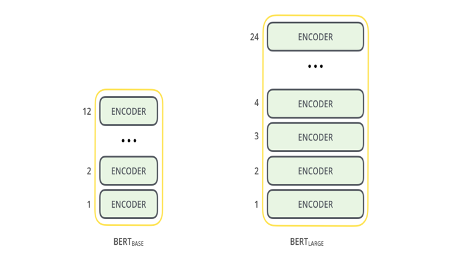
\includegraphics{figures/figure1.png}
	\caption{\label{fig:my-label} BERT base and BERT large \cite{BERT}}
\end{figure}

\begin{figure}[!htbp]
	\centering
	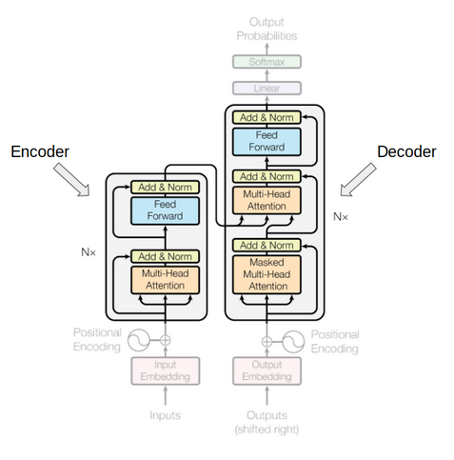
\includegraphics{figures/figure2.png}
	\caption{\label{fig:my-label} Transformer Architecture \cite{attention}}
\end{figure}

\begin{figure}[!htbp]
	\centering
	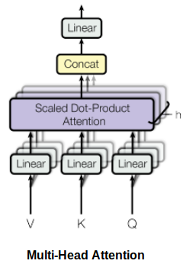
\includegraphics{figures/figure3.png}
	\caption{\label{fig:my-label} Multi-Head Attention \cite{attention}}
\end{figure}

\begin{figure}[!htbp]
	\centering
	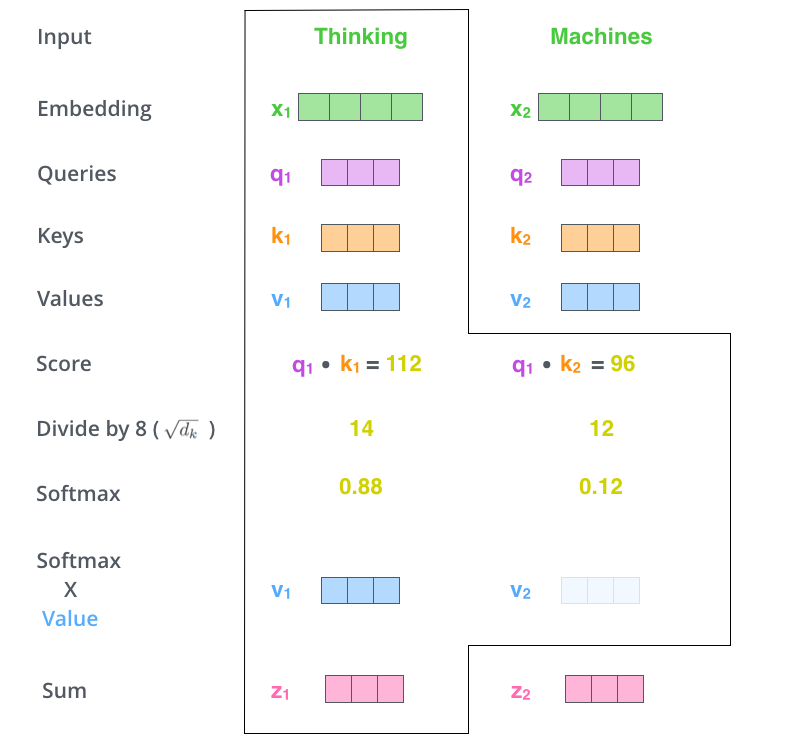
\includegraphics[scale=0.3]{figures/self-attention.png}
	\caption{\label{fig:my-label} Calculate Self-Attention \cite{self-attention}}
\end{figure}


\subsection{Transfer Learning}

Because of how well the BERT models performs, BERT is often combined with transfer learning to solve different NLP tasks. Instead of building a model from scratch, we can use a pre-trained model like BERT to solve our own specific problems, with a little bit fine-tuning to adapt the model. This saves a lot of resources because our model does not need to learn every parameter from scratch. In the case of pre-trained BERT (base), we do not need to learn the first 12 layers of parameters. We can just add a layer on top of them to solve specific problems. \\
\\
BERT is pre-trained on two tasks: Masked Language Modeling (MLM) and Next Sentence Prediction (NSP).
For MLM, before feeding text sequences into BERT, some words in the sequence are masked with the [MASK] token. BERT then tries to predict the original value of the masked words based on the context of the sequence.\\
\\
For NSP, BERT receives pairs of text sequences as input, and BERT tries to predict if the second sentence is the subsequent sentence in the original document.
When the BERT model was trained, both MSM and NSP were trained together, and the goal was to minimize the combined loss function of both.

\subsection{XLM-RoBERTa}

BERT is trained entirely on English data. Many researchers who are working on non-English data have then come up with language specific models such as Finnish BERT, French BERT and German BERT. Research on a multilingual model continues to this day. In November 2019, the Facebook AI team released XLM-RoBERT \cite{xlm-roberta}, an update to their XLM-100 model. They used the RoBERTa \cite{roberta} model (A Robustly Optimized BERT Pretraining Approach) to improve XLM-100 and hence produce XLM-RoBERTa.\\
\\
XLM-RoBERTa is trained on 100 languages, a total of 2.5TB of text. The pre-trained XLM-RoBERTa has 550 million parameters, compared to RoBERTa's 355 million.

\subsection{TPU}

The Tensor Processing Unit is an ASIC developed by Google to specialize in deep learning. Models that previously took days to train on GPU can be trained in hours on TPU. However, in order to use PyTorch on TPU, we have to use a package called Pytorch/XLA. There are currently no stable releases of this platform.

\section{Data}

The Jigsaw Kaggle competition \cite{kaggle} has provided a training set, a validation set, and a test set. The training set’s comments are entirely in English. The validation and test sets' comments are composed of multiple non-English languages, such as, Spanish, French, Italian, Russian, etc. I have combined the training set from the previous competition to make a large training set of 2.1 million comments. Since my computational resources are limited, I only used the first 200,000 datapoints. \\
\\
I used the BERT and XLM-RoBERTa pre-trained tokenizer to tokenize and pad the training data.\\
\\
The validation set has 8,000 datapoints. I tested my trained model directly on the validation set without translating it into English because I want to see how my model is adapting to non-English languages.\\
\\
The test set has 63,812 datapoints. I used this test set shared by one of the competitors \cite{test-en-df} which translates the entire test set into English. I used this translated test set to evaluate my BERT and BERT+CNN models because I want to achieve the best score possible on test set. However,  I evaluated my XLM-RoBERTa model directly on the test set because it is a cross-lingual model.\\ 
\\
Since this is a kernel-only competition, inferencing is done separately on Kaggle notebooks.

\begin{figure}[!htbp]
	\centering
	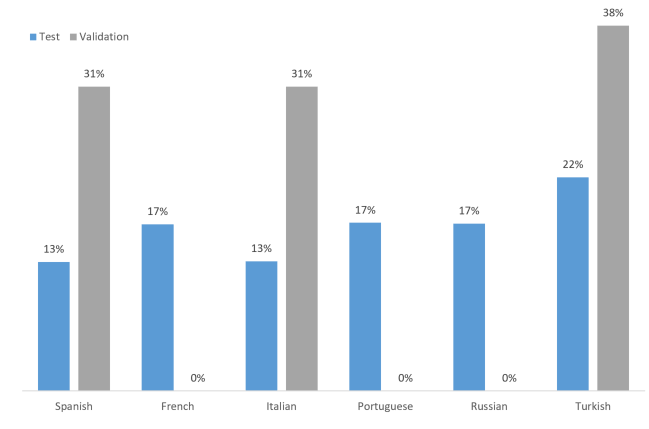
\includegraphics[scale=1.5]{figures/data.png}
	\caption{\label{fig:my-label} Languages used in Validation and Test set}
\end{figure}


\section{Models}

This section  investigates three different models using both GPU and TPU.

\subsection{BERT for Text Classification Directly}

To adapt pre-trained BERT (base) model to classify toxic comments, I simply added a classifier layer on top of the 12 BERT layers. Then, I fine-tuned the hyperparameters to improve performance.\\
\\
First, I added drop out for BERT output to prevent overfitting. The BERT model produces two outputs: last hidden state and pooled output. I applied mean pooling and max pooling on the last hidden state from BERT output. Then, I concatenated them and sent it to a linear (output) layer. \\
\\
The linear (output) layer has size of ($768 \times $2,1). 768 is the hidden size of BERT, which means it has 768 output features, we times it by 2 because we did both max pooling and mean pooling and concatenated them together. Since it is a binary classification problem, I put 1 to make the output value between 0 and 1.\\
\\
I used binary cross entropy with logits loss as the loss function, and Adam with decoupled weight decay \cite{weight} as the optimizer. To evaluate the performance on validation set, I used ROC-AUC score \cite{roc}, which is a desirable way to measure classification performance.  It has the following advantages: (1) It measures how well predictions are ranked, rather than their absolute values. (2) It measures the quality of the model's prediction irrespective of what classification threshold is.\\

\begin{figure}[!htbp]
	\centering
	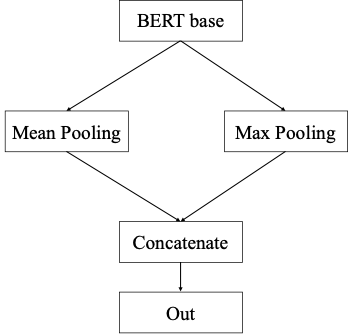
\includegraphics{figures/figure4.png}
	\caption{\label{fig:my-label} BERT for Text Classification}
\end{figure}

\subsection{BERT as word Embeddings + KimCNN}

I used BERT tokenizer to tokenize and pad words into word embeddings. Then I fed them  to a CNN introduced in this paper \cite{kimcnn} by Yoon Kim from New York University in 2014.\\
\\
Here are the steps of how KimCNN works in details \cite{kimcnn}:\\
\\
(1) The word embeddings from BERT are of size [192, 768]. This is because the max sequence length is 192 and the embedding size is 768.\\
\\
(2) The model applies convolution on word embeddings that uses three different filters of size [2, 768], [3, 768], and [4, 768]. These filters correspond to capturing the bi-gram, tri-gram, and 4-gram relations in a sentence.\\
\\
(3) Apply ReLU to add the ability to model nonlinear problems.\\
\\
(4) Apply 1-max pooling to down-sample the output representation of the convolutional layer and to help prevent overfitting.\\
\\
(5) Concatenate vectors after 1-max pooling into a single vector.\\
\\
(6) Dropout (to prevent overfitting).\\
\\
(7) Apply sigmoid function.\\

\begin{figure}[!htbp]
	\centering
	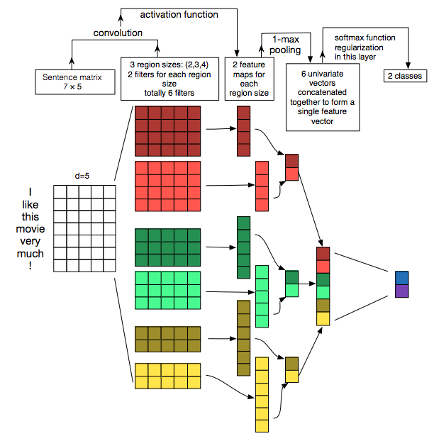
\includegraphics{figures/figure5.png}
	\caption{\label{fig:my-label} KimCNN \cite{kimcnn}}
\end{figure}

\subsection{Cross-lingual model: XLM-RoBERTa}

This is very similar to BERT. The pre-trained XLM-RoBERTa has two outputs, last hidden state and pooled output. The pooled output is fed into a linear (output) layer of size (1024, 1). This is because the hidden size of XLM-RoBERTa is 1024 and the output values should be between 0 and 1.

\section{Experiments}

I have fine-tuned BERT and XLM-RoBERTa to compare against CNN. Also, I have trained BERT both on GPU and TPU to compare the performances.

\subsection{Fine-tune BERT on GPU}

For fine-tuning, I tuned these hyperparameters: learning rate, batch size and number of training epochs.\\
\\
Since the training dataset is rather large and training on GPU takes a long time, I will tune the hyperparameters on the first 50,000 datapoints.\\
\\
The BERT paper had a list of hyperparameters that generally work well across all tasks, which I used as my starting point to fine-tune \cite{BERT}: 
Batch size: 16, 32; Learning rate: 5e-5, 3e-5, 2e-5; Number of epochs: 2, 3, 4.\\
\\
\textbf {Learning Rate:} Learning rate is perhaps the most critical one of all the hyperparameters. To tune learning rate, I fixed the training batch size to be 64 and the validation batch size to be 8. Training on one epoch. The training and validation losses are plotted every 100 batches to make the plots less clustered. I used ROC-AUC score to measure how well my model performed on validation set. Please note that the y-axes of figures below are at different scales. For reference, there are 781 training batches and 1,000 validation batches.\\

\begin{figure}[!htbp]
	\centering
	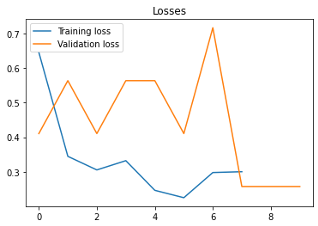
\includegraphics{figures/figure6.png}
	\caption{\label{fig:my-label}  lr = 5e-3}
\end{figure}

\begin{figure}[!htbp]
	\centering
	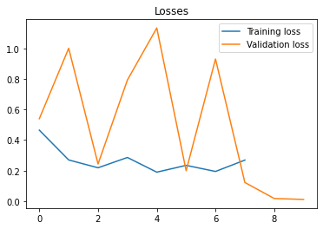
\includegraphics{figures/figure7.png}
	\caption{\label{fig:my-label}  lr = 5e-5}
\end{figure}

\begin{figure}[!htbp]
	\centering
	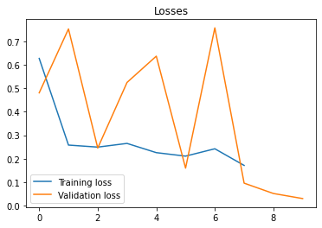
\includegraphics{figures/figure8.png}
	\caption{\label{fig:my-label}  lr = 2e-5}
\end{figure}

\begin{figure}[!htbp]
	\centering
	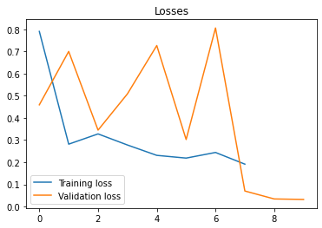
\includegraphics{figures/figure9.png}
	\caption{\label{fig:my-label} lr = 5e-6}
\end{figure}

\begin{table}[!htbp]
	\centering
	\begin{tabular}{|c|c|}
		\hline
		{Learning Rate} & {ROC-AUC} \\ \hline
		5e-3                   & 0.53             \\ \hline
		5e-5                   & 0.82             \\ \hline
		2e-5                   & 0.84             \\ \hline
		5e-6                   & 0.79             \\ \hline
	\end{tabular}
	\caption{\label{table:my-label} Learning Rate vs. ROC-AUC}
\end{table}

\noindent As shown by Table 1, with an aggressive learning rate of 5e-3, the model did poorly on the validation set. I found that a good learning rate for this model should be around 2e-5, which is suggested by the paper.\\

\noindent \textbf {Batch Size:} I set learning rate to be 1e-5, and trained on 3 epochs to tune batch sizes.\\
\\
Generally, too large of a batch size will lead to poor generalization, while too small of a batch size will not guarantee convergence to the global optimum. It will bounce around the global optima instead. \\
\\
I have found that the max training batch size I can use for this model is 64. I tried training batch sizes of 128 and 256, which will blow up the GPU memory on Google Colab notebook.\\

\begin{table}[!htbp]
	\centering
	\begin{tabular}{|c|c|c|}
		\hline
		{Training} & {Validation} & {ROC-AUC} \\ \hline
		16                           & 2                              & 0.79             \\ \hline
		32                           & 4                              & 0.81             \\ \hline
		64                           & 8                              & 0.82             \\ \hline
	\end{tabular}
	\caption{\label{table:my-label} Batch Size vs. ROC-AUC}
\end{table}

\noindent This table shows that training batch size of 64 is ideal for this model given my constraints.\\

\noindent \textbf {Number of Epochs: }  After trained on 6 epochs with learning rate of 1e-6, training batch size of 64, and validation batch size of 8. I got an ROC-AUC score of 0.83 at the 6th epoch.\\
\\
 As the originial paper suggests, BERT is far less sensitive to hyperparameter tuning on large data sets (100k+)\cite{BERT}. The results show that once the hyperparameters are set near the optimal values, it does not affect the performance of the model much.\\
\\
\noindent My fine-tuned BERT (base) model achieved the accuracy of 0.9012 on the test set on Kaggle. This model took 4.7 hours to train on GPU.\\

\begin{table}[!htbp]
	\centering
	\begin{tabular}{|c|c|}
		\hline
		{Max Sequence Length}   & 192  \\ \hline
		{Training Batch Size}   & 64   \\ \hline
		{Validation Batch Size} & 8    \\ \hline
		{Epochs}                & 5    \\ \hline
		{Learning Rate}         & 1e-6 \\ \hline
	\end{tabular}
	\caption{\label{table:my-label} Best Performed BERT}
\end{table}


\subsection{Fine-tune BERT on TPU}

I trained my best BERT model on TPU. I used XLA package, which enables PyTorch on Google TPU. To make the training process even faster, I utilized all 8 cores on TPU to parallel processing. I have trained for one epoch to see how fast the speed up on TPU is.\\

\begin{table}[!htbp]
	\centering
	\begin{tabular}{|c|c|}
		\hline
		{XLA : 1} & 12m 16s \\ \hline
		{XLA : 2} & 12m 12s \\ \hline
		{XLA : 3} & 12m 15s \\ \hline
		{XLA : 4} & 12m 13s \\ \hline
		{XLA : 5} & 12m 18s \\ \hline
		{XLA : 6} & 12m 17s \\ \hline
		{XLA : 7} & 12m 28s \\ \hline
		{XLA : 8} & 12m 19s \\ \hline
	\end{tabular}
	\caption{\label{table:my-label} Training Time on TPU}
\end{table}

\noindent As shown by Table 4, it only took 12 minutes to train for one epoch on TPU vs. 56 minutes to train for one epoch on GPU.\\

\subsection{BERT + CNN}

I started with a relatively large batch size and learning rate training for 5 epochs. Then I gradually tuned down the batch size and learning rate while training for more epochs.\\
\\
However, this model does not perform well on the dataset. The training loss failed to converge to a low loss, and the ROC-AUC score is quite low.\\

\begin{table}[!htbp]
	\centering
	\begin{tabular}{|c|c|c|}
		\hline
		Training Batch Size & Learning Rate & ROC-AUC \\ \hline
		128                 & 1e-3          & 0.51    \\ \hline
		128                 & 1e-5          & 0.44    \\ \hline
		64                  & 5e-6          & 0.46    \\ \hline
		32                  & 1e-6          & 0.44    \\ \hline
	\end{tabular}
	\caption{\label{table:my-label} BERT+CNN}
\end{table}

\subsection{Fine-tune XLM-RoBERTa}

I did similar fine-tuning procedures as the BERT model described above. I found that the max training batch size I can use on Colab TPU is 16.

\begin{table}[!htbp]
	\centering
	\begin{tabular}{|c|c|c|}
		\hline
		Learning Rate                & ROC-AUC & Time    \\ \hline
		5e-6  & 0.9394  & 46m 7s  \\ \hline
		1e-6   & 0.9552  & 43m 36s \\ \hline
	\end{tabular}
	\caption{\label{table:my-label} Learning Rate vs. ROC-AUC}
\end{table}

\noindent After fine-tuned XLM-RoBERTa, my best performed model achieved 0.9459 on test set on Kaggle.

\begin{table}[!htbp]
	\centering
	\begin{tabular}{|c|c|}
		\hline
		{Max Sequence Length}   & 192  \\ \hline
		{Training Batch Size}   & 16   \\ \hline
		{Validation Batch Size} & 4    \\ \hline
		{Epochs}                & 2    \\ \hline
		{Learning Rate}         & 5e-6 \\ \hline
	\end{tabular}
	\caption{\label{table:my-label} Best Performed XLM-RoBERTa}
\end{table}


\section{Conclusion}

I have found that transfer learning utilizing BERT is very effective compared to using a simple model such as CNN. A large language model like BERT takes a lot of resources to train and it generalizes very well on many NLP tasks, including text classification. On the other hand, the CNN model I tried is very simple and did not have enough data to be trained on.\\
\\
Transfer learning also depends on the similarity between the task the model was trained on and the task that needs to be solved. Since XLM-RoBERTa was trained to be a cross-lingual model, it generalizes well on the test set than BERT, which is a mono-lingual model.\\
\\
Therefore, transfer learning utilizing BERT to do text classification will achieve a high performance without a lot of effort compared to building a specific model from scratch, which is quite challenging.\\
\\
Lastly, TPU is powerful especially when it comes to training a very large model like BERT. Models like BERT and XLM-RoBERTa take a lot of computational resources to train. TPU dramatically increases the speed of training those models.\\

\newpage
\bibliography{final_report}\
\bibliographystyle{plain}

\end{document}
